\documentclass[notitlepage, oneside]{report}
\usepackage[utf8]{inputenc}
\usepackage{polski}
\usepackage{amsmath}
\usepackage{fancyhdr,lipsum}
\usepackage{graphicx,lastpage}
\usepackage{etoolbox}
\fancypagestyle{plain}{
  \fancyhf{}
  \fancyhead[R]{
\includegraphics[width=\linewidth,height=55pt]{ppbuam.png}}}
\pagestyle{plain}

\usepackage{titling}


\begin{document} 
\vline\break
\begin{center}
\section*{{\LARGE Podpisy biometryczne na tablecie i ich porównanie  z podpisami na papierze}}
\section*{{\Large Raport końcowy}}

{\Large Mikołaj Balcerek (lider zespołu) \\ Bartosz Hejduk \\ Mieczysław Krawiarz \\ Adam Kulczycki \\ Mikołaj Pabiszczak \\ Michał Szczepanowski \\ Dawid Twardowski \\ Adrianna Załęska \\}
   
\section*{Poznań, wrzesień 2017}
\end{center}

\chapter*{Wprowadzenie}
 \section*{Wstęp}
 Zrealizowany projekt dotyczył zbierania i analizy podpisów biometrycznych. Dynamiczny podpis biometryczny służy weryfikacji tożsamości osoby go składającej. Weryfikacja odbywa się na podstawie porównania cech uśrednionego podpisu wzorcowego (składa się nań zwykle ca. 5 podpisów) z cechami podpisu składanego. Pośród cech, które mogą być brane pod uwagę wyróżnia się m.in.:
 \begin{itemize}
 	\item kształt graficzny podpisu, w tym kształt liter;
 	\item właściwości fizyczne sygnatury, rozmiar pociągnięć oraz czas ich złożenia;
 	\item nacisk jaki pióro wywiera na powierzchnię pisania i jego zmienność w czasie;
 	\item ruchy wykonywane piórem podczas pisania - szybkości i przyspieszenia pióra w kierunkach ustalonych osi współrzędnych, jak również liczba oderwań pióra od powierzchni pisania;
 	\item położenie pióra względem płaszczyzny pisania -  kąt pisania i jego zmiany w czasie.
 \end{itemize}

 Powyższe cechy nie są jednakowe w każdej chwili w czasie składania podpisu, stąd algorytmy weryfikacji analizują zbliżoność rozkładu tychże cech w czasie („górki i dołki występować winny w analogicznej kolejności i wielkości, jednakże być może w nieco różnych odległościach od siebie”). Algorytmy weryfikacji mogą bazować m.in. Ukrytych Modelach Markowa (ang. \textit{Hidden Markov Models}) czy Dynamicznym Marszczeniu Czasu (ang. \textit{Dynamic Time Warping}).

 Porównywanie podpisów odbywa się w sposób przybliżony. Efektem porównania jest ocena w postaci punktacji lub procentu określająca podobieństwo złożonych podpisów. Ustalenie progu, decydującego o zaklasyfikowanie podpisu jako prawdziwego, dopuszcza pewien poziom błędu, którego uwzględnienie decyduje o fałszywym odrzuceniu prawdziwego podpisu (ang. \textit{False Rejection}) i o fałszywym przyjęciu nieprawdziwego podpisu (ang. \textit{False Acceptance}).
\section*{Zakres projektu}
Projekt obejmował stworzenie aplikacji do zbierania i weryfikacji podpisów składanych na urządzeniu \textit{Microsoft Surface} przy użyciu pióra \textit{Microsoft Surface Pen} wraz z opracowaniem algorytmu weryfikacji i stworzeniem bazy danych podpisów (obejmującej podpisy wzorcowe, podpisy prawdziwe i fałszywe), na podstawie której testowano stworzone algorytmy weryfikacji podpisów dynamicznych.

\chapter*{Model fizyczny}
\section*{Aplikacja}
Aplikacja \textit{Podpis Biometryczny} składa się z programu \textbf{PodpisBio} oraz wspierającej go bazy danych.
\section*{Program}
     Program \textbf{PodpisBio} został zorganizowany w dwa główne podfoldery, \textit{Src} oraz \textit{View}.
     
     Podfolder \textit{View} zawiera implementację graficznego interfejsu użytkownika i jest podzielony na osobne podstrony, takie jak stronę składania podpisów (\textit{SignaturePage.xaml}) lub stronę z danymi statystycznymi (\textit{StatisticPage}).
     
 W podfolderze \textit{Src} znajduje się główna implementacja projektu. Dzieli się ona na subfoldery \textit{Author}, \textit{FinalScore} oraz \textit{Service}. Ostatni z nich zajmuje się łączeniem i aktualizowaniem projektu z lokalną bazą danych podpisów.
 
 W  \textit{Author} znajdziemy klasę implementującą Autora (\textit{Author.cs}) oraz jej kontroler. Pozwala to na przypisanie podpisów do różnych autorów i rozróżnianie pomiędzy nimi. Dalej, implementację klasy Sygnatura (\textit{Signature.cs}), przechowującą i zajmującą się obsługą sygnatur. Pomocnicze klasy Punkt oraz Pociągnięcia (\textit{Point.cs}, \textit{Stroke.cs}) dzielą podpis na pomniejsze jego części i są przechowywane jako listy. Klasy \textit{TimeSizeProbe.cs} oraz \textit{Dynamics.cs} badają odpowiednio zależności rozmiaru podpisu do czasu jego złożenia (dla całej sygnatury jak i również dla osobnych pociągnięć) oraz przyspieszenia i szybkości poruszeń pióra \textit{Microsoft Surface Pen}.
 
   Folder \textit{FinalScore} zawiera klasy zajmujące się określaniem finalnego stopnia pewności w autentyczność podpisu oraz metodę DTW (\textit{Dynamic Time Warping}).
   
    Klasy i foldery pomocniczne \textit{Weight}, \textit{FileController}, \textit{RealScreenSizeCalculator} zajmują się odpowiednio obliczaniem wag poszczególnych metod weryfikacji podpisu, zapisywaniem podpisów w formie graficznej i w pliku .csv, oraz obliczaniem rzeczywistego pola podpisu na podstawie informacji o przekątnej ekranu oraz jego rozdzielczości.
    



\chapter*{Model logiczny - zrealizowane funkcjonalności}

\begin{figure}
\centering
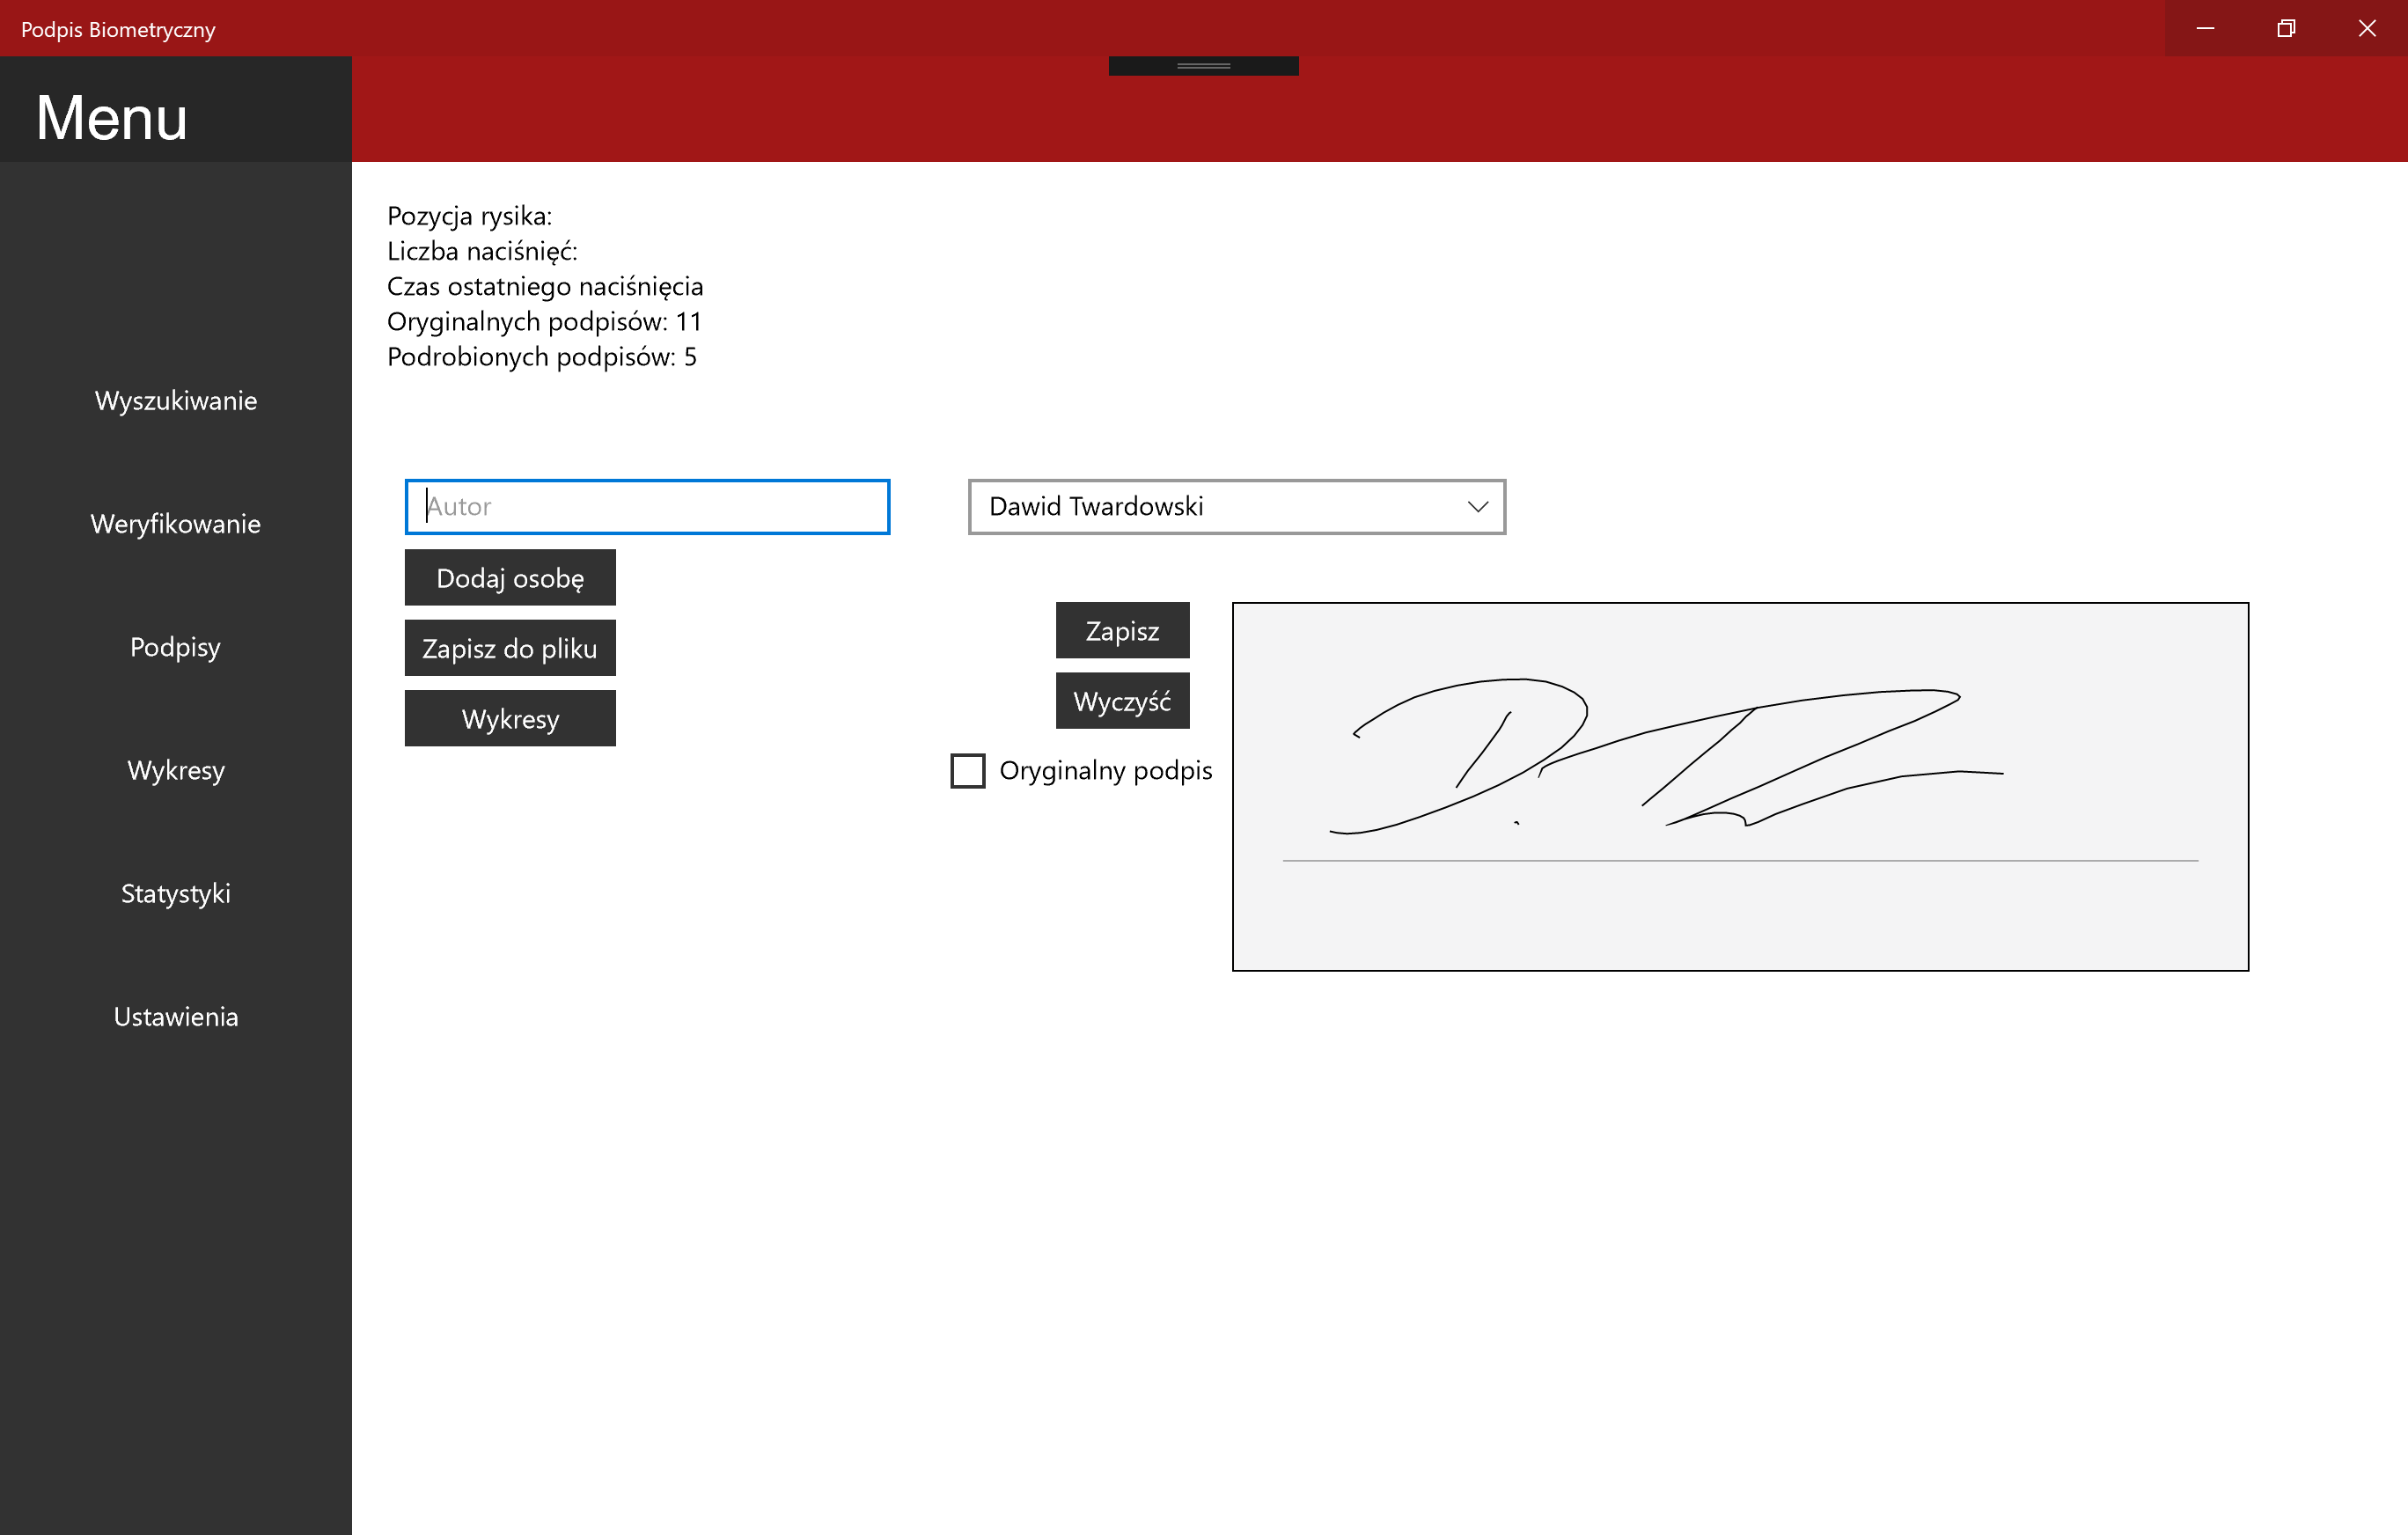
\includegraphics[width=12cm]{oknopodpis.PNG}
\caption{Okno podpisu, tutaj można złożyć podpis dla zaznaczonego autora, spróbować go podrobić oraz zapisać do plików}
\label{rys:Okno podpisu w aplikacji}
\end{figure}

\section*{Składanie podpisu}
\begin{itemize}
  \item rejestracja podpisu - informacje zawierające jego fizyczny rozmiar, szybkości, przyspieszenia, siłę naciśnięć rysika oraz czas złożenia podpisu;
  \item pole składania podpisu dynamicznie zmieniające rozmiar w zależności od przekątnej i rozdzielczości wykorzystywanego ekranu, tak by zachować wymagane pole ok. 110mm x 40mm;
  \item pole składania podpisu zawierające pomoce (linie wodzące) oraz możliwość wycofania podpisu;
  \item obsługa gumki znajdującej się na końcu \textit{Microsoft Surface Pen} jako wycofania podpisu;
  \item zarządzanie listą autorów, synchronizowaną z bazą danych;
  \item możliwość przyporządkowania podpisów do danego autora;
  \item określanie prawdziwości lub fałszywości podpisu w trakcie jego dodawania do bazy danych;
  \item opcjonalna pomoc w tworzeniu fałszywych podpisów w formie nakładki oryginalnego podpisu w polu do pisania;
  \item synchronizacja bazy autorów i podpisów z lokalną bazą danych.
 \end{itemize}
 
 \section*{Pogląd podpisów}
 
 \begin{figure}
\centering
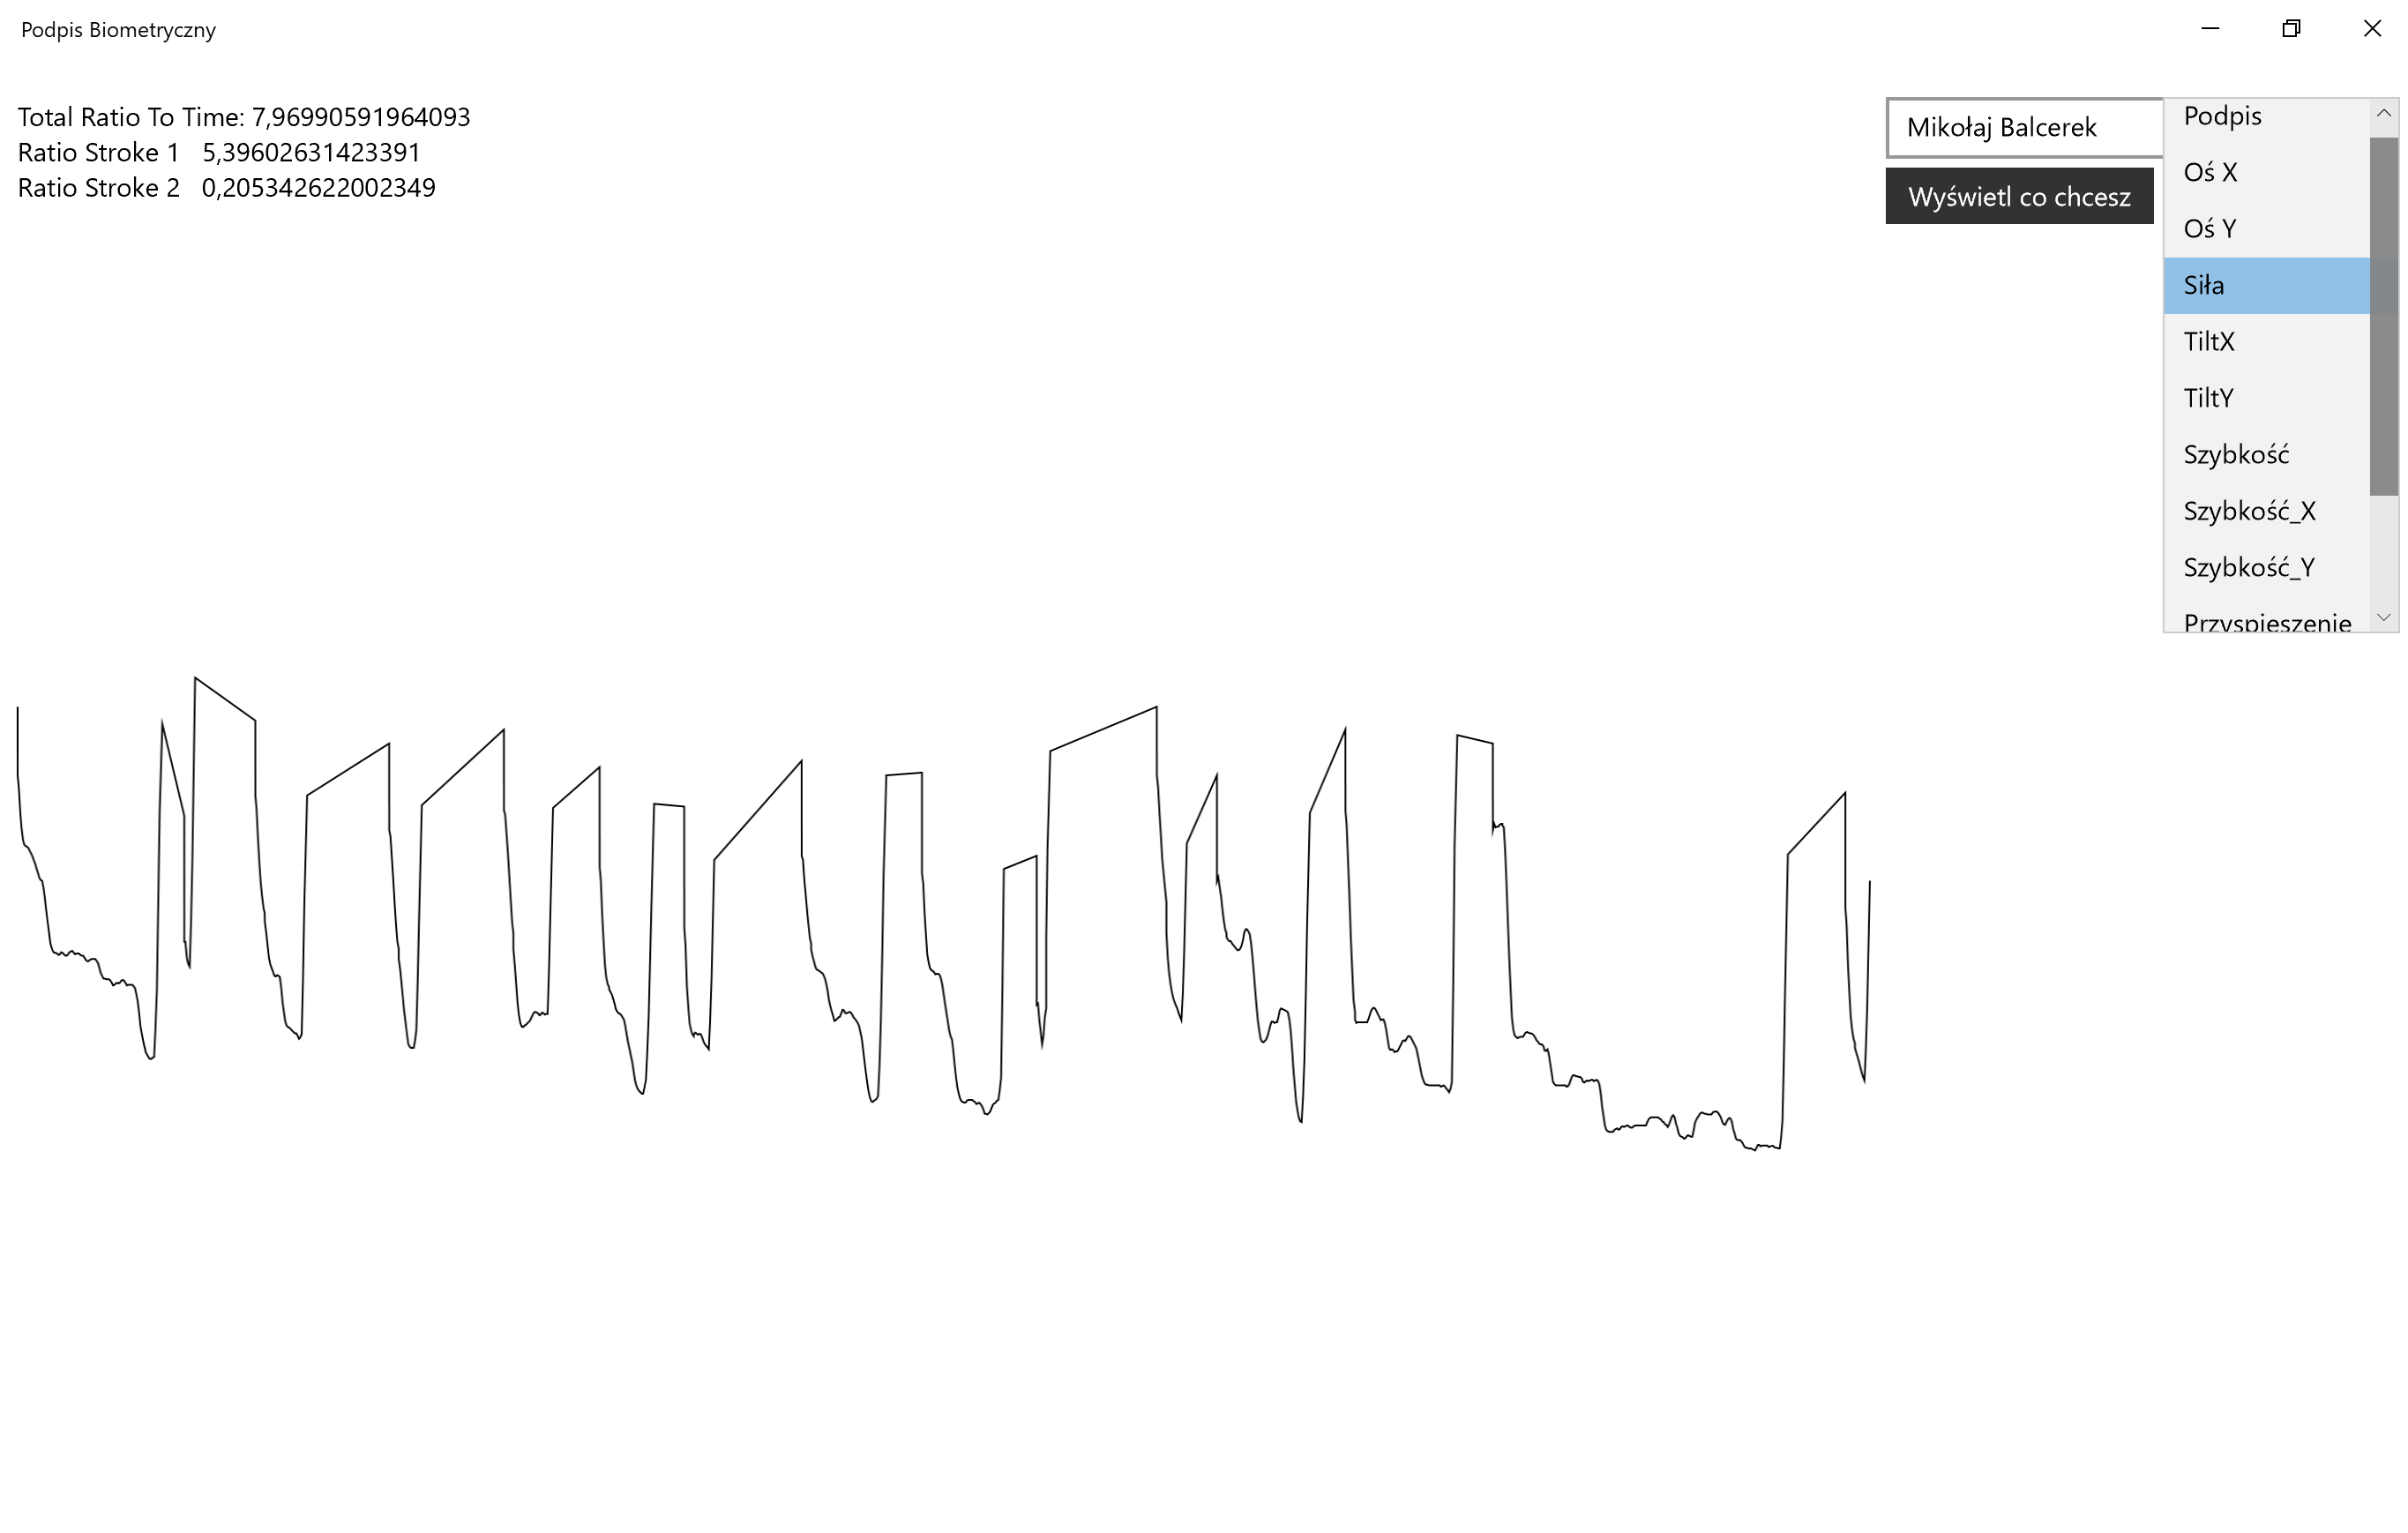
\includegraphics[width=12cm]{oknowykres.png}
\caption{Okno poglądu sygnatur z bogatymi opcjami generowania wykresów na podstawie różnych zebranych danych}
\label{rys:Okno wykresów w aplikacji}
\end{figure}

\begin{itemize}
  \item możliwość wyświetlania podpisów dla wszystkich autorów znajdujących się w bazie danych;
  \item pogląd metryk TimeSize dla podpisów z osobna;
  \item pogląd wykresów przyspieszeń, przyspieszeń w osiach, szybkości, szybkości w osiach oraz sił naciśnięć;
  \item zapisywanie podpisów do plików graficznych .gif;
  \item zapisywanie podpisów w formie niezmodyfikowanej do plików .csv.
 \end{itemize}
 \section*{Normalizacja podpisów}
\begin{itemize}
  \item wszystkie złożone podpisy są skalowane do stałych rozmiarów, tak by mimo różnic w rozmiarze rzeczywistym były one łatwe do porównania;
  \item podpisy po złożeniu są odpowiednio centrowane i przesuwane tak, by wszystkie sygnatury zaczynały się w jednym punkcie i nie zawierały luk.
 \end{itemize}
\section*{Możliwości weryfikacji podpisu}

 \begin{figure}
\centering
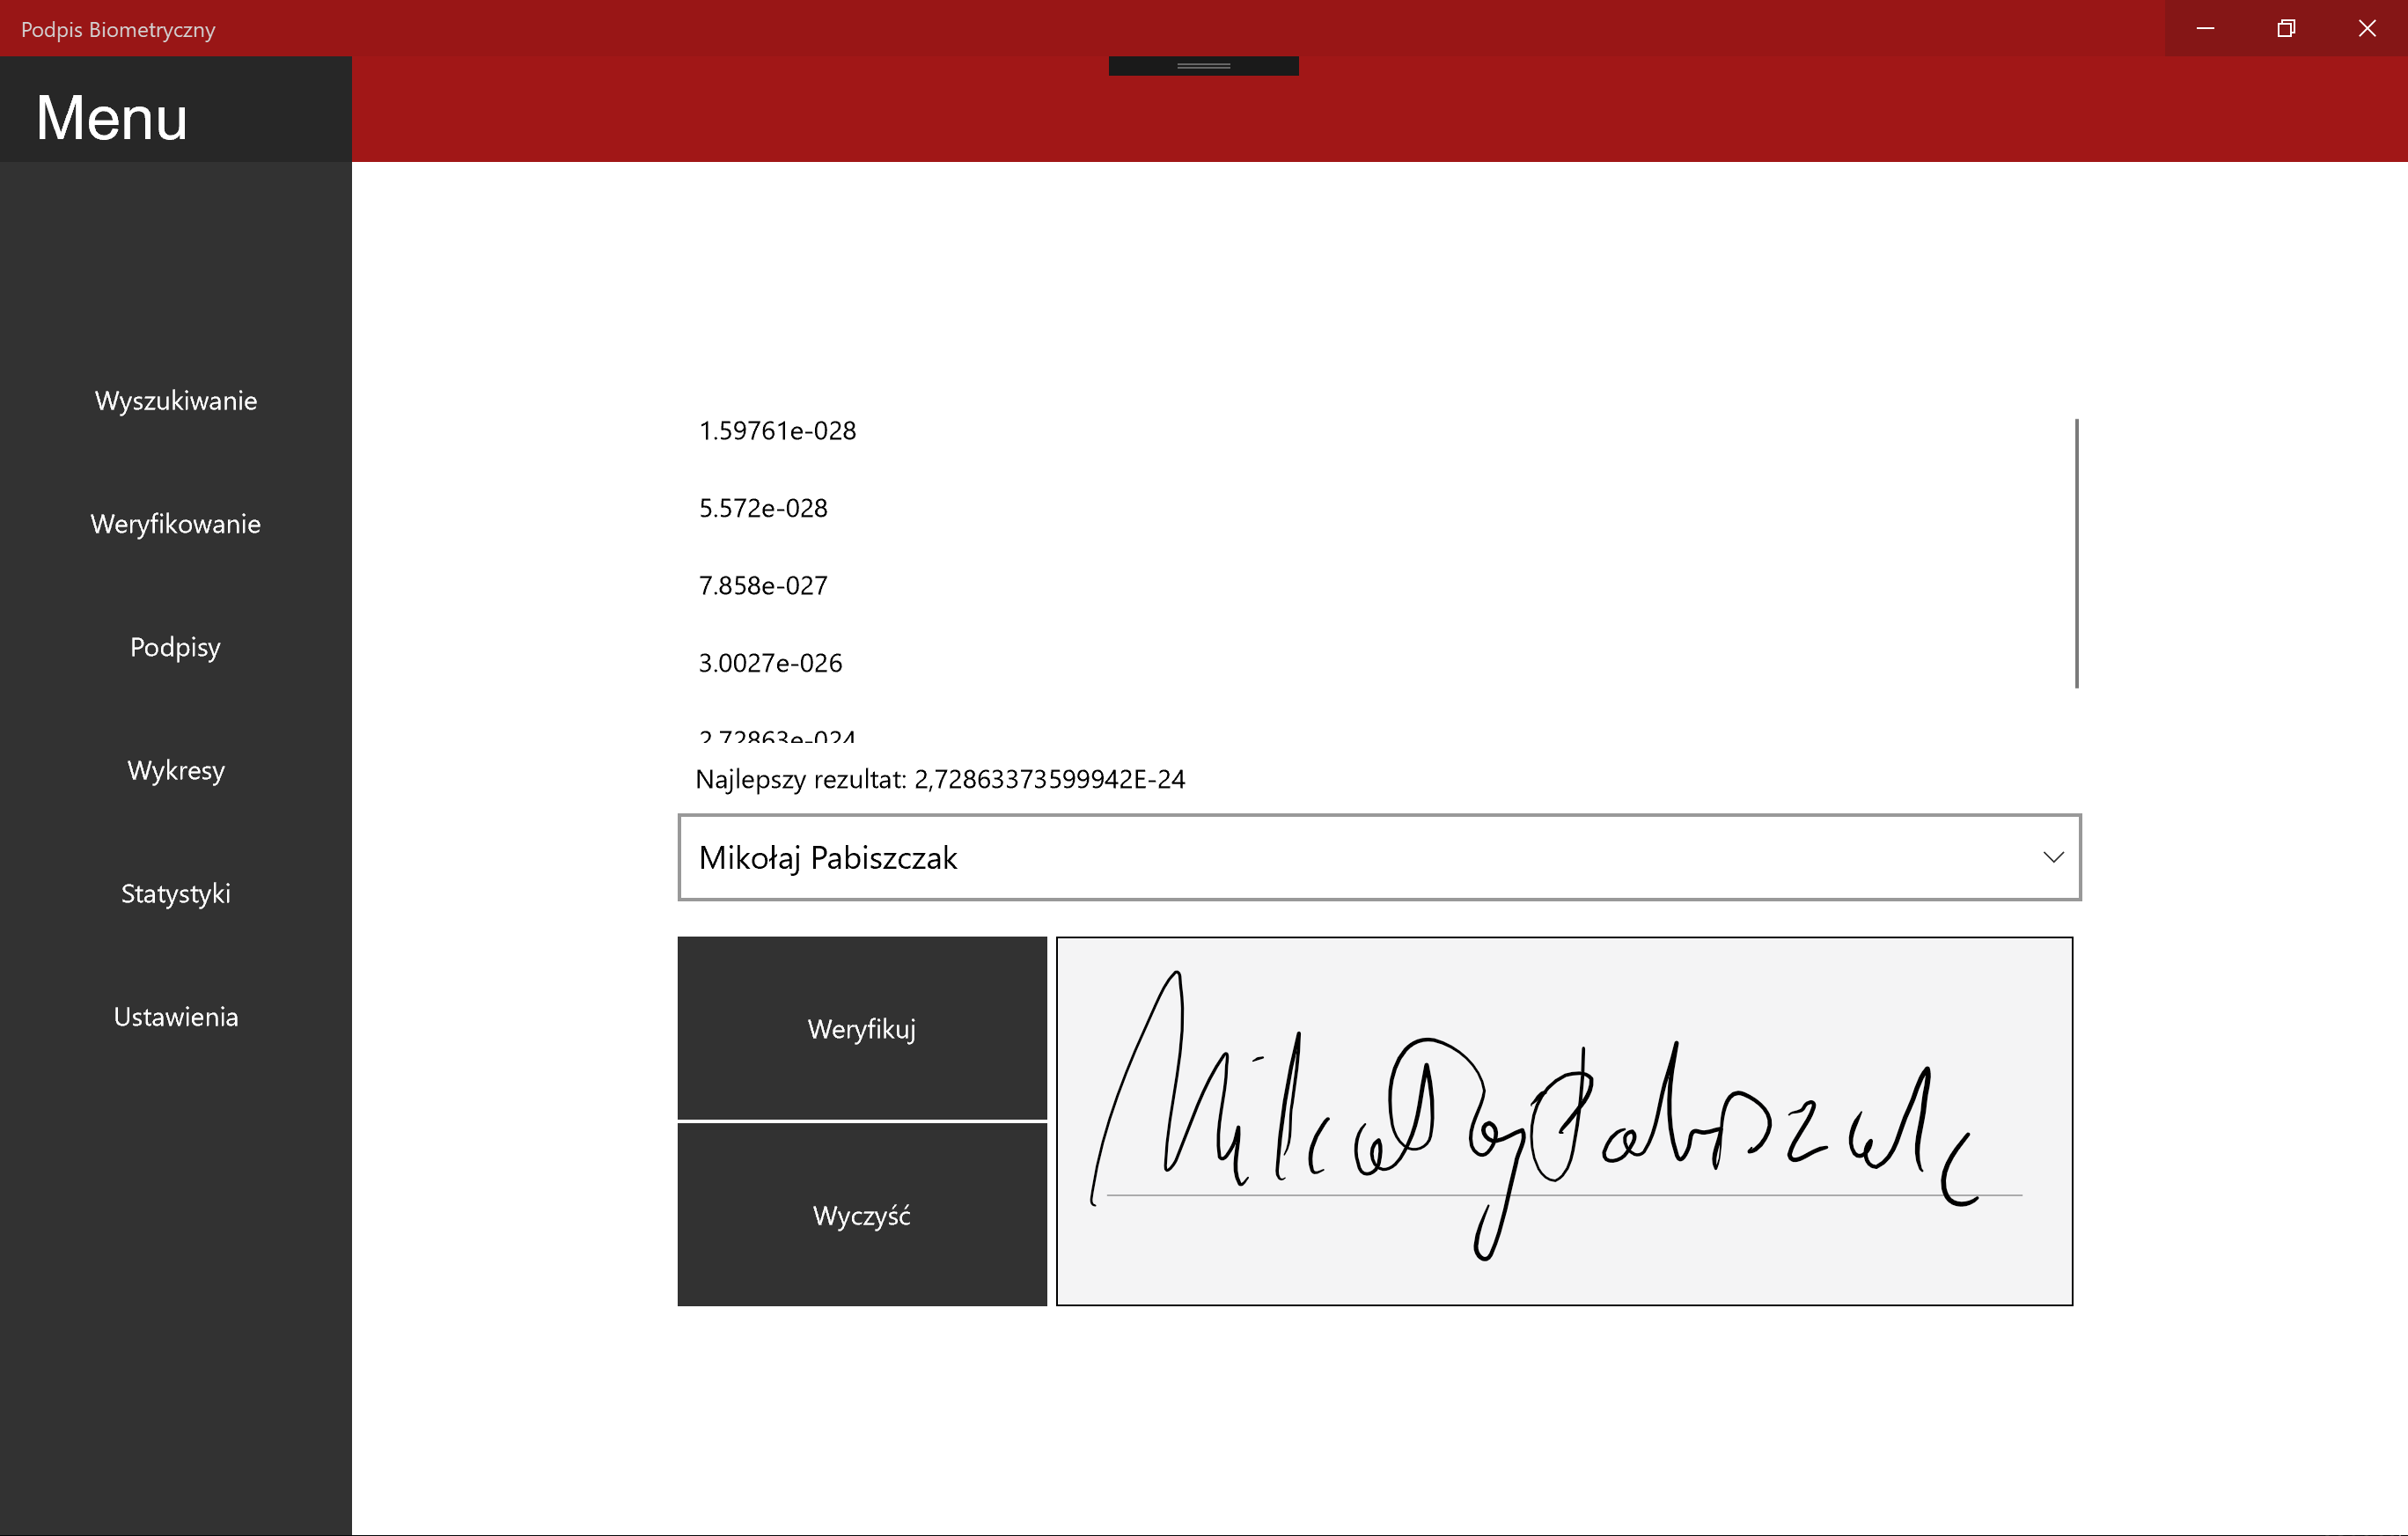
\includegraphics[width=12cm]{oknoweryfikacji.PNG}
\caption{Składanie sygnatur i pogląd wyników autentykacji. Złożony na rysunku fałszywy podpis słusznie otrzymuje bardzo niski wynik pewności na poziomie ok. 0,00.....3}
\label{rys:Okno weryfikacji sygnatury}
\end{figure}

\begin{itemize}
  \item weryfikowanie podpisów na podstawie stosunku rozmiaru całego podpisu do czasu jego złożenia (rzeczywistego czasu wodzenia rysika po ekranie);
  \item szybkie odrzucanie podpisów zbyt krótkich lub znacząco za długich w obydwu osiach;
  \item sprawdzanie autentyczności sygnatur korzystając ze stosunku rozmiarów (wykorzystanego wirtualnego "atramentu") osobnych pociągnięć do czasu rzeczywistego ich złożenia;
  \item określanie autentyczności podpisu na podstawie funkcji zmian siły nacisku (czy siła nacisku maleje, jest stała czy rośnie w czasie);
  \item badanie podpisów metodą Dynamic Time Warping, biorącą pod uwagę współrzędne, przyspieszenia, szybkości oraz siły nacisku podpisu;
  \item możliwość przypisywania wag dla poszczególnych metod badania autentyczności podpisu;
  \item wczesna wersja przypisywania indywidualnej ważności poszczególnych metod weryfikacji dla każdego użytkownika z osobna;
 \end{itemize}
 \section*{Badanie skuteczności programu}
 
  \begin{figure}
\centering
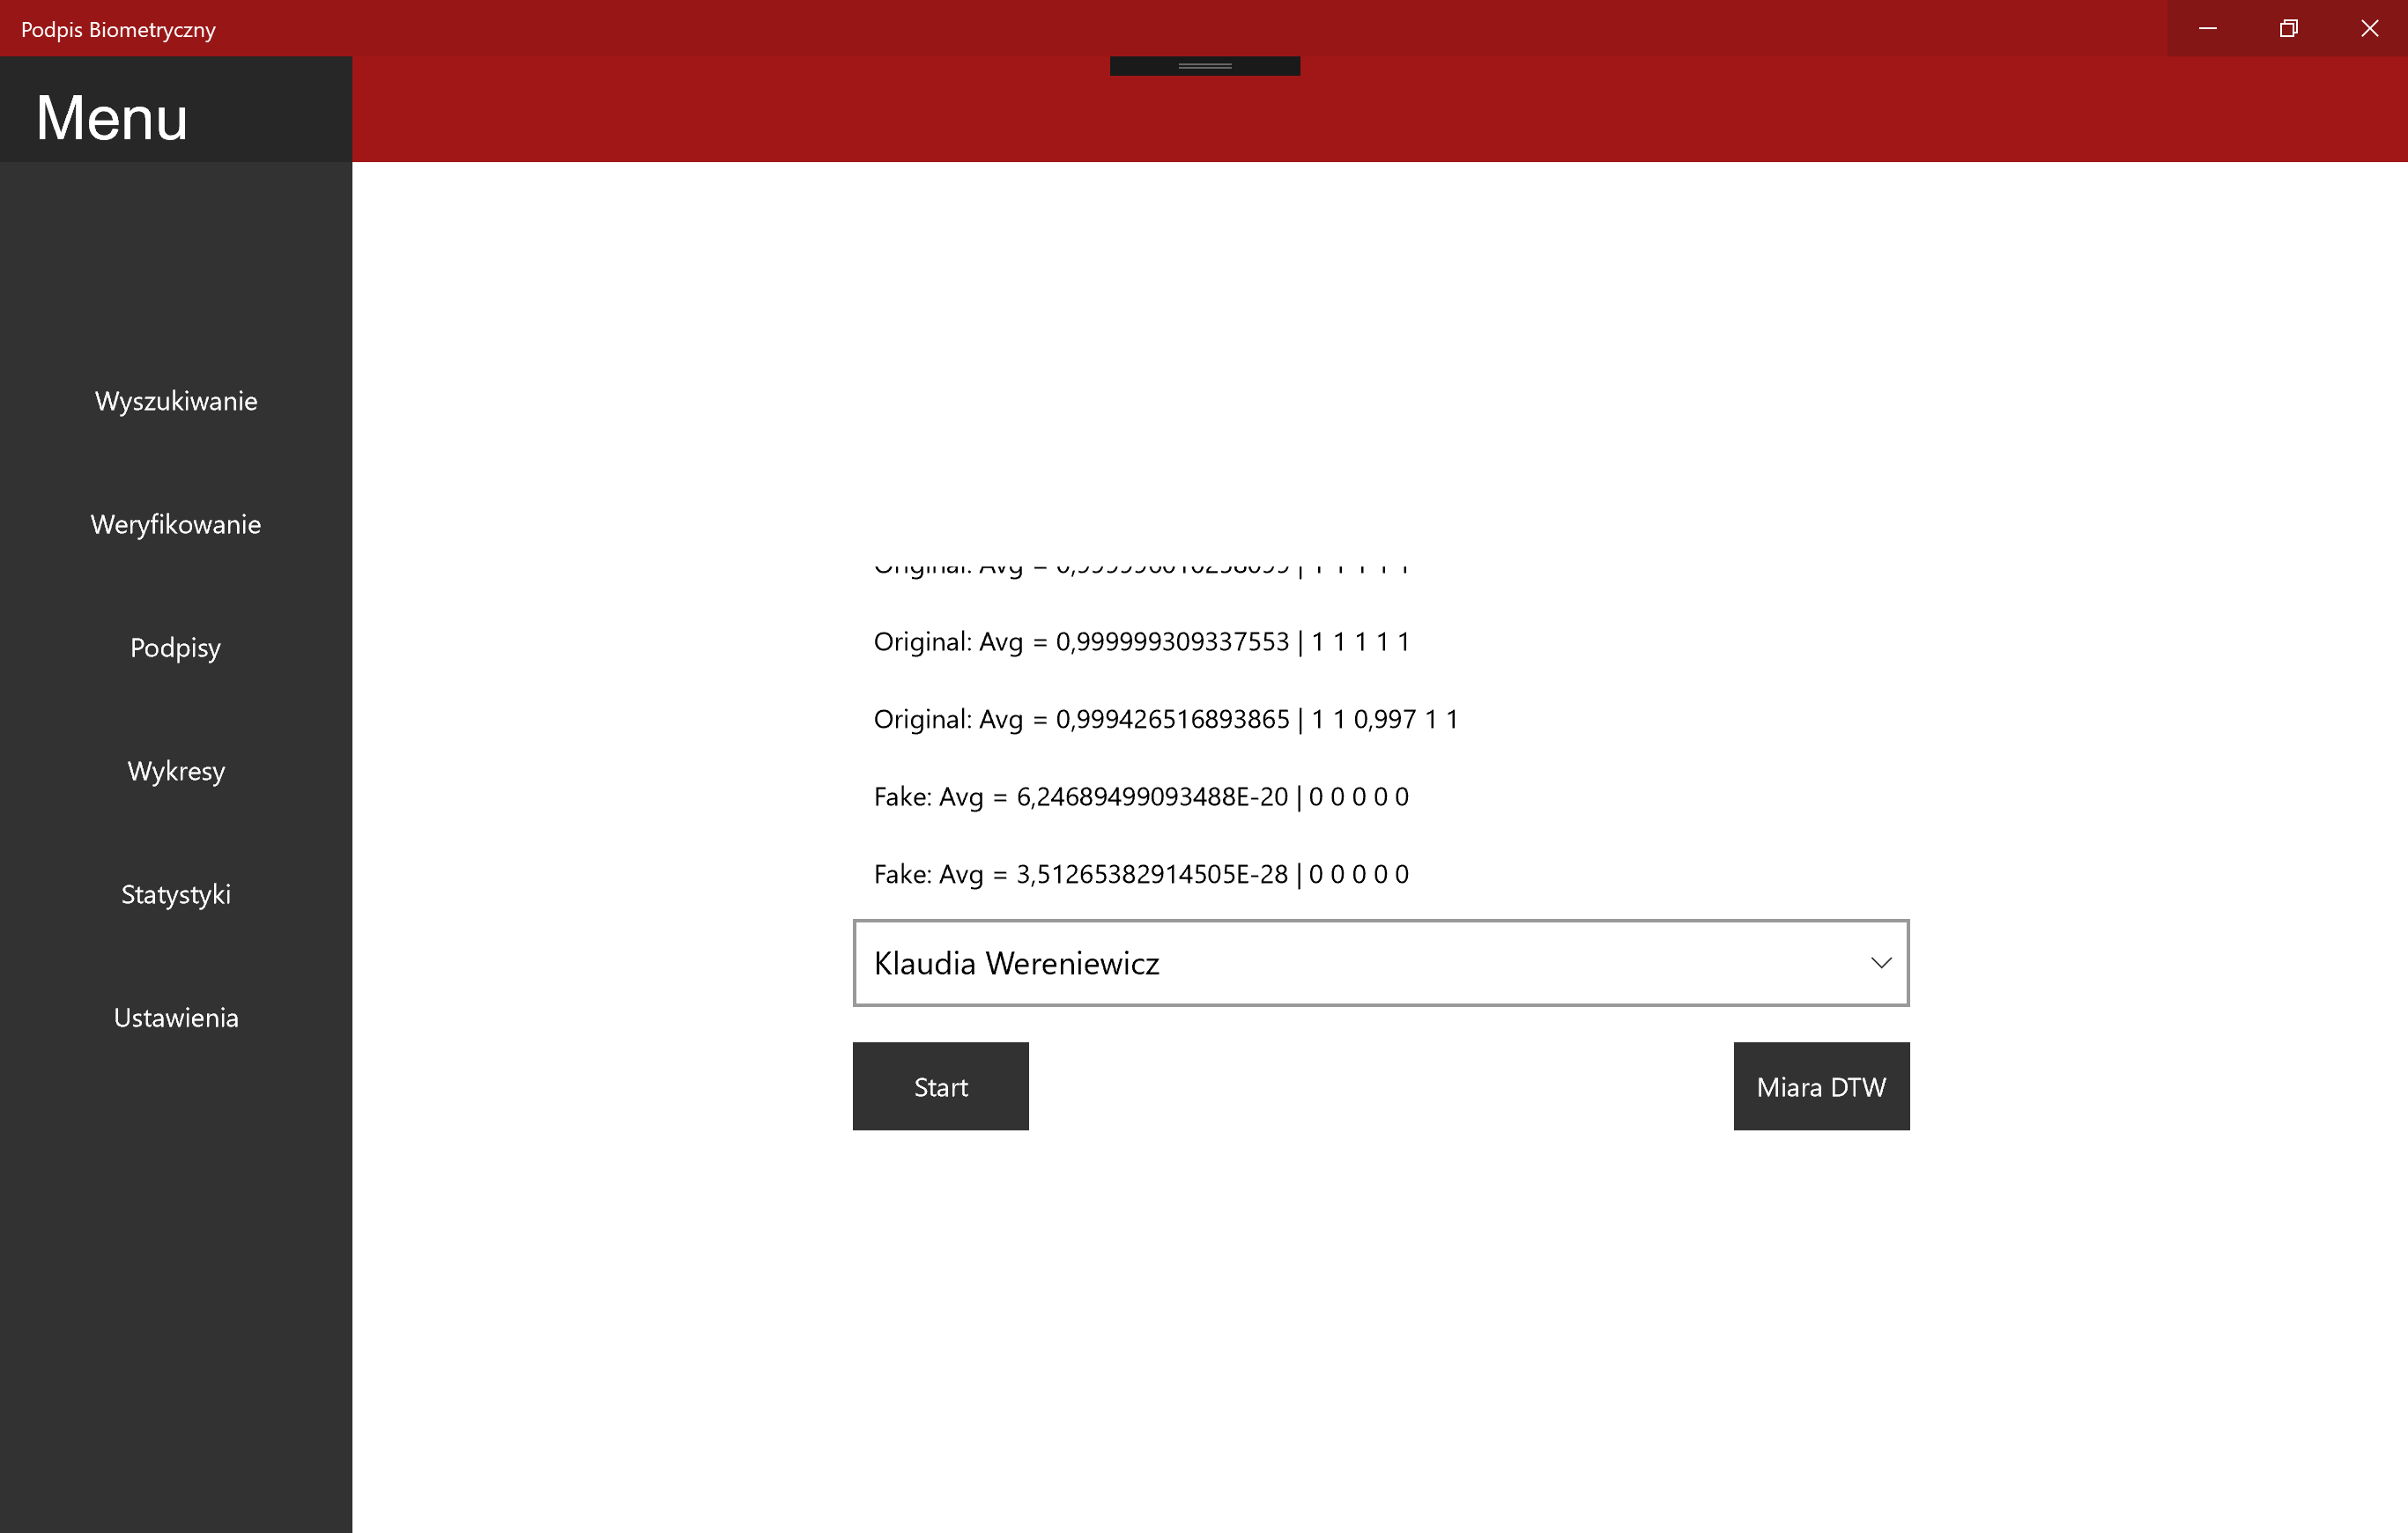
\includegraphics[width=12cm]{statystyki.PNG}
\caption{Pogląd wyników weryfikacji dla wszystkich podpisów złożonych w imieniu danej osoby. Szczególnie warto zwrócić uwagę na wysoką pewność podpisów oryginalnych na poziomie 0,999.. w porównaniu z niską autentycznością sygnatur fałszywych (0,00....6)}
\label{rys:Okno weryfikacji sygnatury}
\end{figure}

\begin{itemize}
  \item osobna strona pozwalająca na szybkie testowanie metod weryfikacji wobec wybranej osoby;
  \item finalny wynik weryfikacji jako liczba 0-1 określająca prawdopodobieństwo prawdziwości składającego podpis;
  \item nauka algorytmów wzorca podpisu danej osoby na podstawie tylko 3-5 podpisów
  \item określanie prawdopodobieństwa autentyczności zarówno prawdziwych jak i fałszywych podpisów na podstawie wybranych pięciu wzorcowych podpisów.  
  \item strona ze wstępnymi informacjami statystycznymi;
  \item badanie skuteczności wszystkich metod wobec wiadomego statusu oryginalny/fałszywy podpisu dla danego autora;  
  \item wysoka skuteczność  i dokładność metody \textit{DTW}, słusznie określająca fałszywość sygnatur dla większości sygnatur, z możliwością określenia wyniku do 30+ miejsc po przecinku
 \end{itemize}

\chapter*{Opis środowiska}
\section*{Użyte technologie}
Program \textit{Podpis Biometryczny} został wykonany w języku programowania \textbf{C\#}, wykorzystując technologię \textit{Universal Windows Platform}. Zastosowanie tej bazy ułatwia dostęp do informacji o pozycji \textit{Microsoft Surface Pen} oraz ogólnym wykorzystaniu ekranu dotykowego. Aplikacje \textit{Universal Windows Platform} w łatwy sposób dostosowują się do pracy na telefonach, tabletach oraz komputerach osobistych. Wymagają jednak korzystania wyłącznie z platformy  \textit{Windows 10}.

Serwer z bazą danych oparty jest na technologii \textbf{.NET Framework} w wersji 4.6.1. W bazie przechowywane są podpisy oraz ewentualne parametry, których obliczanie każdorazowo byłoby nieefektywne.



\chapter*{Algorytmy weryfikacji podpisów}


 \section*{Współczynniki bezpieczeństwa w biometrii}
 W biometrii porównuje się cechy przynajmniej dwóch wzorców cech biometrycznych - pierwszy pobierany jest podczas rejestracji użytkownika w systemie, drugi zaś na bieżąco podczas weryfikacji. O ile cechy biometryczne pozostają niezmienne, to wzorce tych samych cech biometrycznych pobierane w różnym czasie są różne. Stąd w przypadku, gdy porównywane wzorce są identyczne można stwierdzić, iż ma miejsce próba nieuprawnionego uwierzytelnienia (oszustwa). Weryfikacja polega na porównywaniu podobieństwa dwóch wzorców. Wynikiem porównywania jest zazwyczaj punktacja lub wyrażona w procentach zgodność wzorców. Przyjęcie odpowiedniego progu (w punktach lub procentach) umożliwia zaklasyfikowanie składanego wzorca jako prawdziwego lub fałszywego; ponadto próg taki można regulować zmieniając wiarygodność uwierzytelniania. \\
 
Miarami wiarygodności uwierzytelniania są współczynniki:
  \begin{itemize}
      \item fałszywej akceptacji osoby nieuprawnionej (ang. FAR - \textit{False Acceptance Rate});
      \item fałszywego odrzucenia osoby uprawnionej (ang. FRR - ang. \textit{False Rejection Rate});
      \item równowagi błędów (ang. EER - ang. \textit{Equal Error Rate}).
  \end{itemize}
  
\begin{figure}
\centering
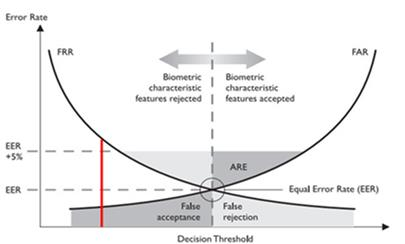
\includegraphics[width=12cm]{Biometrics-Error-Rates.jpg}
\caption{Graficzne przedstawienie FAR, FRR, ERR. (Żródło: ISC2, International Information Systems Security Certification Consortium)}
\end{figure}



  
  Fałszywa akceptacja zachodzi, gdy algorytm klasyfikuje podpis osoby nieuprawnionej za prawdziwy; fałszywe odrzucenie - gdy podpis osoby uprawnionej zostaje zaklasyfikowany jako fałszywy. W praktyce jako parametr porównywania skuteczności różnych metod weryfikacji stosuje się EER - im niższy, tym metoda jest lepsza. \\
  
  Współczynniki te oblicza się następująco:
  \begin{equation*}
      FAR = \frac{liczba falszywie zaakceptowanych}{liczba prob weryfikacji}
  \end{equation*}
  \begin{equation*}
      FRR = \frac{liczba falszywie odrzuconych}{liczba prob weryfikacji}
  \end{equation*}

 \section*{Zaimplementowany algorytm}
 Algorytm na wejściu przyjmuje podpis do weryfikacji, listę podpisów wzorcowych danego autora (vide algorytm ustalania wag) oraz wagi dla danego autora. Na~wyjściu zwraca informację o tym, czy podpis przeszedł weryfikację.
 \begin{enumerate}
 \item Dla każdego z podpisów wzorcowych wykonuje się kroki 2-4.
 \item Dla każdego ustalonego parametru oblicza się podobieństwo tego parametru pomiędzy podpisem do weryfikacji, a podpisem wzorcowym. \\
 W przypadku DTW wykorzystuje się również próg DTW dla danego autora do obliczenia podobieństwa.
 \item Wyniki z kroku poprzedniego mnoży się przez wagę odpowiadającą danemu parametrowi.
 \item Sumuje się wyniki dla poszczególnych parametrów.
 \item Z otrzymanej listy wybiera się maksimum, które na podstawie określonej metryki określa czy podpis przeszedł weryfikację.
 \end{enumerate}


 \section*{Algorytm ustalania wag}
 Algorytm na wejściu przyjmuje listę podpisów oryginalnych. Na~wyjściu zwraca wagi dla ustalonych parametrów oraz próg dla DTW.
 \begin{enumerate}
 \item Bierze się pierwsze \textbf{x} podpisów jako podstawę do wyliczenia wag (\textbf{x} ustalone - w naszym przypadku 5).\\Jeżeli \textbf{x} jest większe od liczby otrzymanych podpisów to wszystkie traktuje się jako podstawę.
 \item Dla ustalonych parametrów oblicza się ich podobieństwo \mbox{(przedział od 0 do 1)} na podstawie podpisów uznanych za bazowe.\\(1 = (odchylenie standardowe / średnia))
 \item Przy obliczaniu podobieństwa dla DTW zapisuje się również próg~\mbox{(~=~średnia)} dla danego autora.
 \item Wyniki z kroku 2 dla ważniejszych parametrów mnoży się ponadto przez stałą (ustaloną bądź wyliczoną).
 \item Wagą dla danego parametru jest wynik podzielony przez sumę wyników dla wszystkich parametrów.
 \end{enumerate}
 
% \section*{Dynamic Time Warping}

\chapter*{Czego nie udało się zrealizować}
Pośród rzeczy, których nie udało nam się (w całości) zrealizować (z różnych powodów) są:
 \begin{itemize}
  \item funkcjonalność dokładnego odrzucania podpisów, które wykroczyły poza pole wprowadzania. Ten feature został zrealizowany częściowo.;
  \item pobieranie formularza od IC Solutions i wykrywania pola wprowadzania podpisu na skanie kartki (np. wniosku o założenie konta w banku). Potrzeba na tą możliwość została zasygnalizowana na późnym etapie projektu ;
  \item zbieranie informacji o kątach pisania;
  \item dopracowanie algorytmów weryfikacji i stworzenie algorytmów opartych na innych metodach (np. Ukrytych Modelach Markowa, probabilistyczne DTW);
  \item resampling szeregów czasowych;
  \item wyznaczenie stałego progu dla akceptacji podpisu (dla każdego autora wyznaczany jest indywidualny próg na podstawie 5 podpisów wzorcowych);
  \item stworzenie statystyk dla różnych algorytmów, które pomogłyby w ich porównywaniu.
 
 \end{itemize}
 
 \chapter*{Kod źródłowy oraz uruchamianie aplikacji}
  \section*{Wersje programu}
  Najnowszą przetestowaną wersję programu można ściągnąć z {https://github.com/MikolajBalcerek/PodpisBio/releases}.
 \section*{Kod źródłowy i dane}
 Kod źródłowy aplikacji znajduje się na repozytorium pod adresem: \\
 \url{https://github.com/MikolajBalcerek/PodpisBio}. \\
 \section*{Uruchomianie aplikacji}
Do uruchomienia programu wymagana jest praca na platformie \textit{Windows 10 Creators Update} lub wyższej, z zainstalowanym IDE \textit{Microsoft Visual Studio} z modułami \textit{Universal Windows Apps} i obsługą języka C\#. Przy pierwszej kompilacji przydatny też jest dostęp do Internetu do automatycznego ściągania pozostałych bibliotek przez środowisko. \\
    W folderze \textit{Program} znajdują się dwa projekty \textit{Visual Studio}, \textit{PodpisBio} oraz \textit{RestService}
 Obydwa są wymagane do uruchomienia projektu. \\ Przed uruchomieniem projektu należy z głównego katalogu \textit{Baza Danych} rozpakować znajdujące w paczce \textit{.zip} pliki \textit{.mdf} oraz \textit{.ldf} i przekopiować je do ścieżki \textit{RestService \textbackslash App\_Data} by uniknąć błędów pobierania wpisów z bazy danych.
  
 
 
 
 

\begin{figure}
\centering
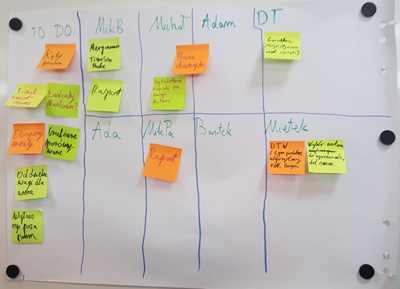
\includegraphics[width=12cm]{karteczki.jpg}
\caption{Dzienny podział pracy w zespole}
\label{rys:karteczki}
\end{figure}

\chapter*{Bibliografia}
\begin{enumerate}
    \item \url{https://github.com/MikolajBalcerek/PodpisBio}
     \item Putz-Leszczyńska J., ,,Biometryczna identyfikacja tożsamości. Biometria podpisu odręcznego"
     \item Plucińska M., ,,Krótki przegląd technik biometrycznych do rozpoznawania osób"
     \item Al-Hmouz R., Pedrycz W., Daqrouq K., Morfeq A., Al-Hmouz A.,  ,,Quantifying dynamic time warping distance using probabilistic model in verification of dynamic signatures"
     \item Llimona Torras Q., ,,Dynamic Time Warping"
     \item Woszczyński T., Marcinkowski Z., Sudoł M. (red.), ,,Raport biometryczny 2.0. Bankowość biometryczna"
    \item Saeed K., Adamski M., ,,Klasyfikacja podpisu offline z wykorzystaniem metody DTW"
    \item Kudłacik P., Porwik P., ,,A new approach to signature recognition using the fuzzy method"
    \item Goc M., ,,Badania podpisów w kryminalistycznej analizie pismoznawczej - wybrane zagadnienia metodyczne"
    \item Hamornik J., ,,Signature-based User Authentication"
    \item Porwik P., Para T., ,,Some Handwritten Signature Parameters in Biometric Recognition Process"
    \item Zwiernik P., ,,Wstęp do ukrytych modeli Markowa i metody Bauma-Welcha"
    \item \url{https://www.tractica.com/biometrics/in-biometrics-which-error-rate-matters/}
    \item \url{http://www.biometria.sk/en/principles-of-biometrics.html}
    \item \url{https://www.quora.com/How-can-I-understand-the-EER-Equal-Error-Rate-and-why-we-use-it}
    \item \url{https://math.stackexchange.com/questions/1292231/what-is-a-decision-threshold-and-how-does-it-apply-to-a-statistical-power}

\end{enumerate}



\end{document}